\chapter{Nitrite Reduction in \Nm{}}

Modelling nitrite reduction involves growing NsrR deficient cultures in aerobic conditions. This mutant expresses AniA and NorB in a constitutive manner, removing the necessity for growing the cultures in microaerobic conditions. The cultures are grown for 3-4 hours after which the culture is added to the electrode chamber and Sodium Nitrite added to a concentration of 1mM.

In the model, Equations (\ref{eq:nitrite} \& \ref{eq:active_ania}) are now also involved, allowing parametrisation of kinetic rates of AniA. This experimental dataset does not unfortunately describe how the concentration of NO changes while Nitrite is being reduced. The prior probability distributions used for this dataset were the posteriors generated from the Nitric Oxide Reduction dataset described above, in accordance with Bayesian inference. The unknown parameters were given non-zero values with flat priors, allowed to burn-in and were then used to generate posterior probability distributions.

A representative dataset and solved output is shown in figure \ref{fig:no2sim}. 

\begin{figure}[ht!]
 \centering
 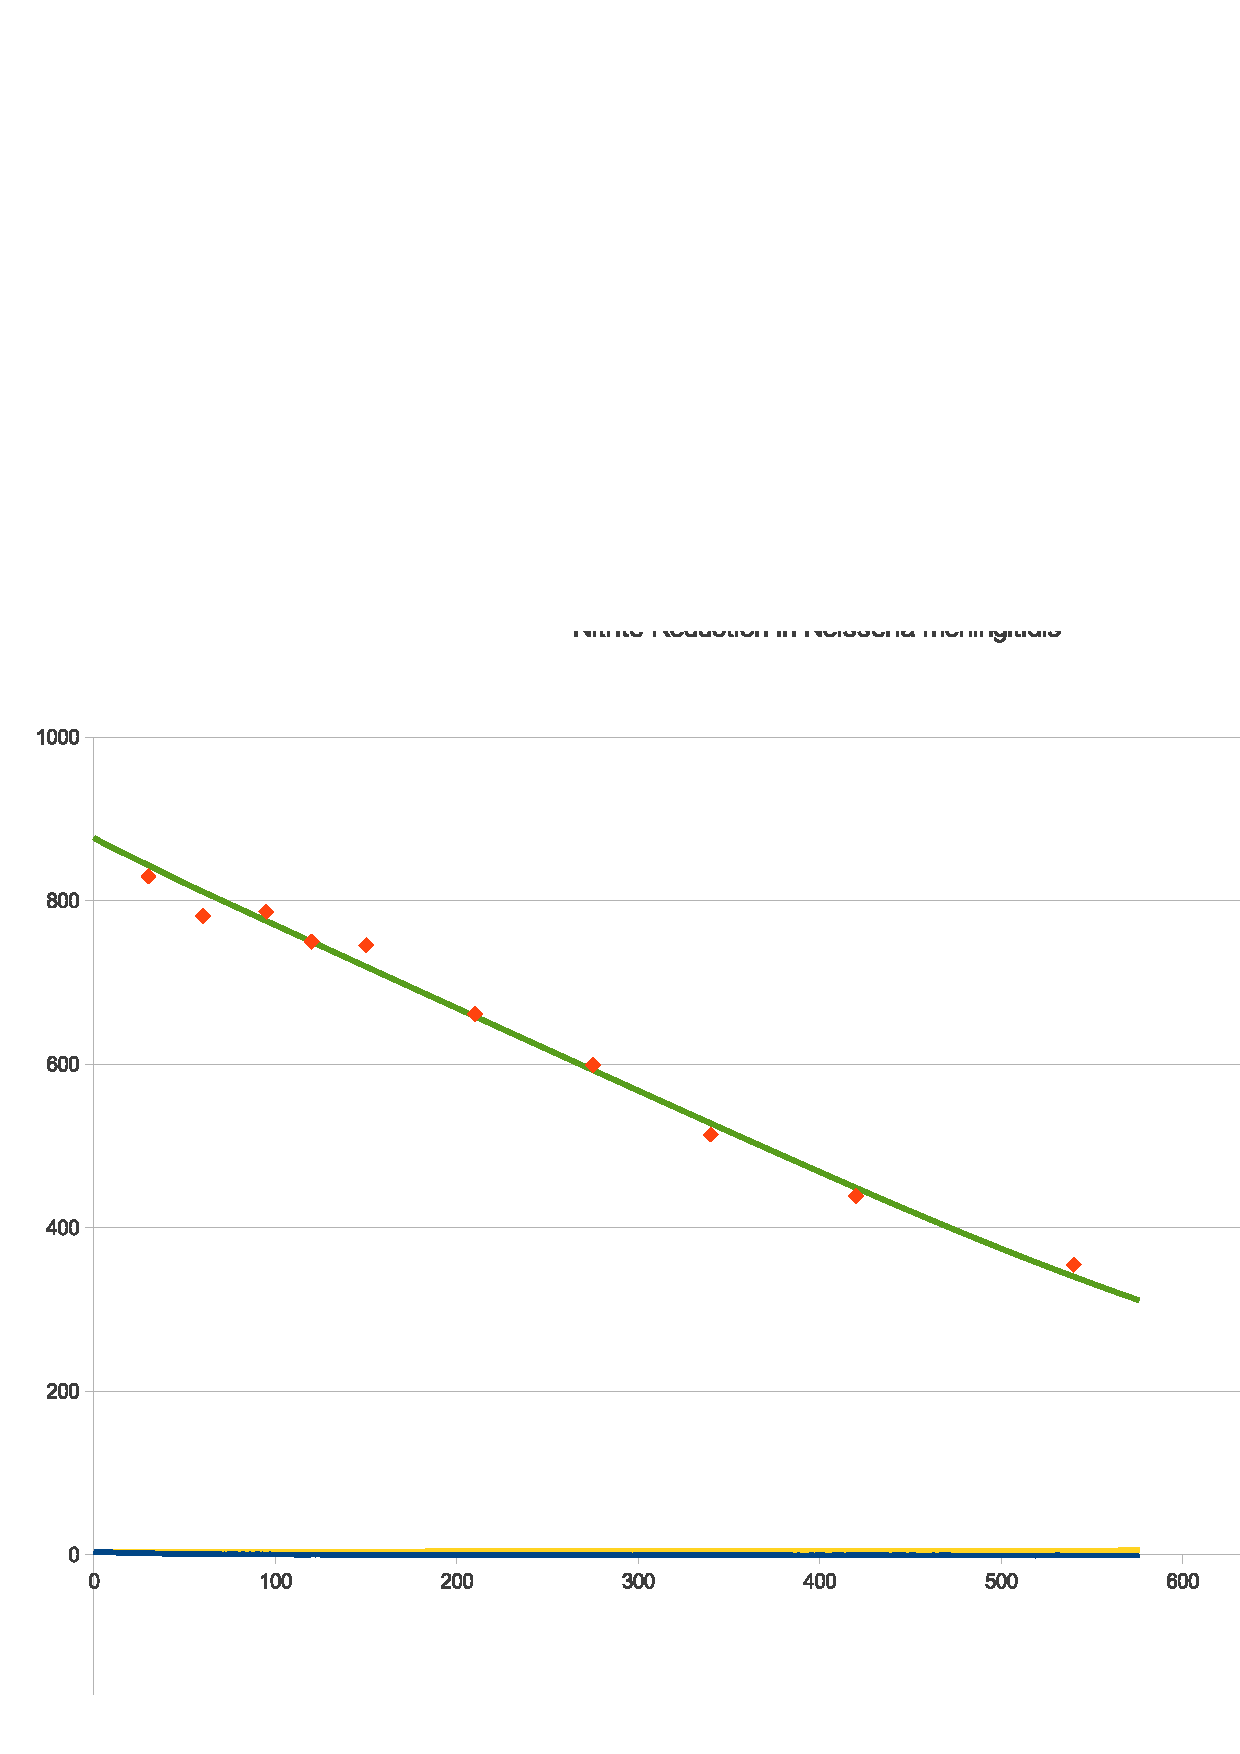
\includegraphics[width=14cm]{./07-nitritereduction/data/no2sim.pdf}
 % no2sim.eps: 0x0 pixel, 300dpi, 0.00x0.00 cm, bb=0 0 785 539
 \caption[{Nitrite Reduction in \textit{Neisseria meningitidis}.}]{{\bf Nitrite Reduction in \textit{Neisseria meningitidis}.} This dataset shows the rate of nitrite reduction when cultures have been grown in microaerobic conditions. The concentrations of nitrite were measured off-line leading to discontinuous data, however the solved output closely matches the experimental data for nitrite.}
 \label{fig:no2sim}
\end{figure}

This is a simpler dataset than for Nitric oxide reduction as it only describes nitrite reduction, along with a small change in oxygen concentration. In combination with prior probability distributions from the afore mentioned dataset it means that the possible values for the kinetic rates involved are automatically going to be limited to those that work alongside the given priors. Without the prior probability distributions the posterior distributions would have a similar outcome to that of the first dataset used, where simple oxygen reduction was modelled, i.e. very wide distributions.

%In the case of this dataset, nitrite reduction has been modelled very well, but nitric oxide (and to a small extent, oxygen) has not been [Caveat, this may change when the cluster does eventually spit out the complete trajectory. This then could be moved into the discussion about why priors are important]. Not shown in Figure \ref{fig:no2sim} is the concentration of nitric oxide as nitrite is reduced. Unfortunately the parameter set used to generate the solved output assigned a very low value to the concentration of NorB (even though this should have been being expressed), thus the nitric oxide produced by reduction of nitrite does not itself get reduced, and towards the end of the dataset would be lethal to the culture. In this case, a different prior distribution should have been used for NorB concentration, as it was known beforehand that NorB concentration would be non-zero. This is an example of why the prior distributions are important.

\section{Microerobic Nitrite Reduction}
\subsection{Introduction}
\subsection{Results}
\subsection{Discussion}
\section{Microaerobic Nitrite Reduction in \textit{norB$^\textrm{-}$} mutant}
\subsection{Introduction}
\subsection{Results}
\subsection{Discussion}
\section{Aerobic Nitrite Reduction in \textit{nsrR$^\textrm{-}$} mutant}
\subsection{Introduction}
\subsection{Results}
\subsection{Discussion}
\section{Aerobic Nitrite Reduction in \textit{nsrR$^\textrm{-}$-norB$^\textrm{-}$} mutant}
\subsection{Introduction}
\subsection{Results}
\subsection{Discussion}